\chapter{Технологическая часть}

В этой части будут указаны средства реализации, листинги с реализациями спроектированных алгоритмов, описан графичесий интерфейс и результаты проведенного тестирования программного обеспечения.

\section{Выбор средств реализации}

В качестве языка программирования был выбран \textit{С++}~\cite{cpp} по ряду причин:
\begin{enumerate}[label=\arabic*)]
	\item В стандартной библиотеке языка присутствует поддержка всех структур данных, выбранных по результатам проектирования;
	\item Средствами языка можно реализовать все алгоритмы, выбранные в результате проектирования.
\end{enumerate}

В качестве среды разработки был выбрана среда $Qt Creator$ вместе с $Qt$~\cite{qt}, так как у него есть встроенные функции для создания пользовательского интерфейса и встроенный отладчик.
Для тестирования был выбран фреймворк \textit{GoogleTest}~\cite{gtest}, так как я уже использовала его ранее.
Для измерения времени будут использоваться функции  \textit{std::chrono::system\_clock::now(...)} и \textit{$std::chrono::duration_cast<std::chrono::milliseconds>$} из библиотеки $chrono$~\cite{cpp-lang-chrono}.

В качестве формата входного файла с фламинго был выбран формат $obj$~\cite{obj}, так как это распространенный формат для хранения 3D объектов.

%\section{Реализация разработанного ПО}

%В листинге (\ref{lst:zb}) представлена реализация модифицированного алгоритма z-буфера,  а в листинге (\ref{lst:refl}) реализация алгоритма для отображения отражений.
\section{Графический интерфейс программы}

Пример пользовательского интерфейса представлен на рисунке (\ref{fig:inter}).
	
\begin{figure}[h!]
	\centering
	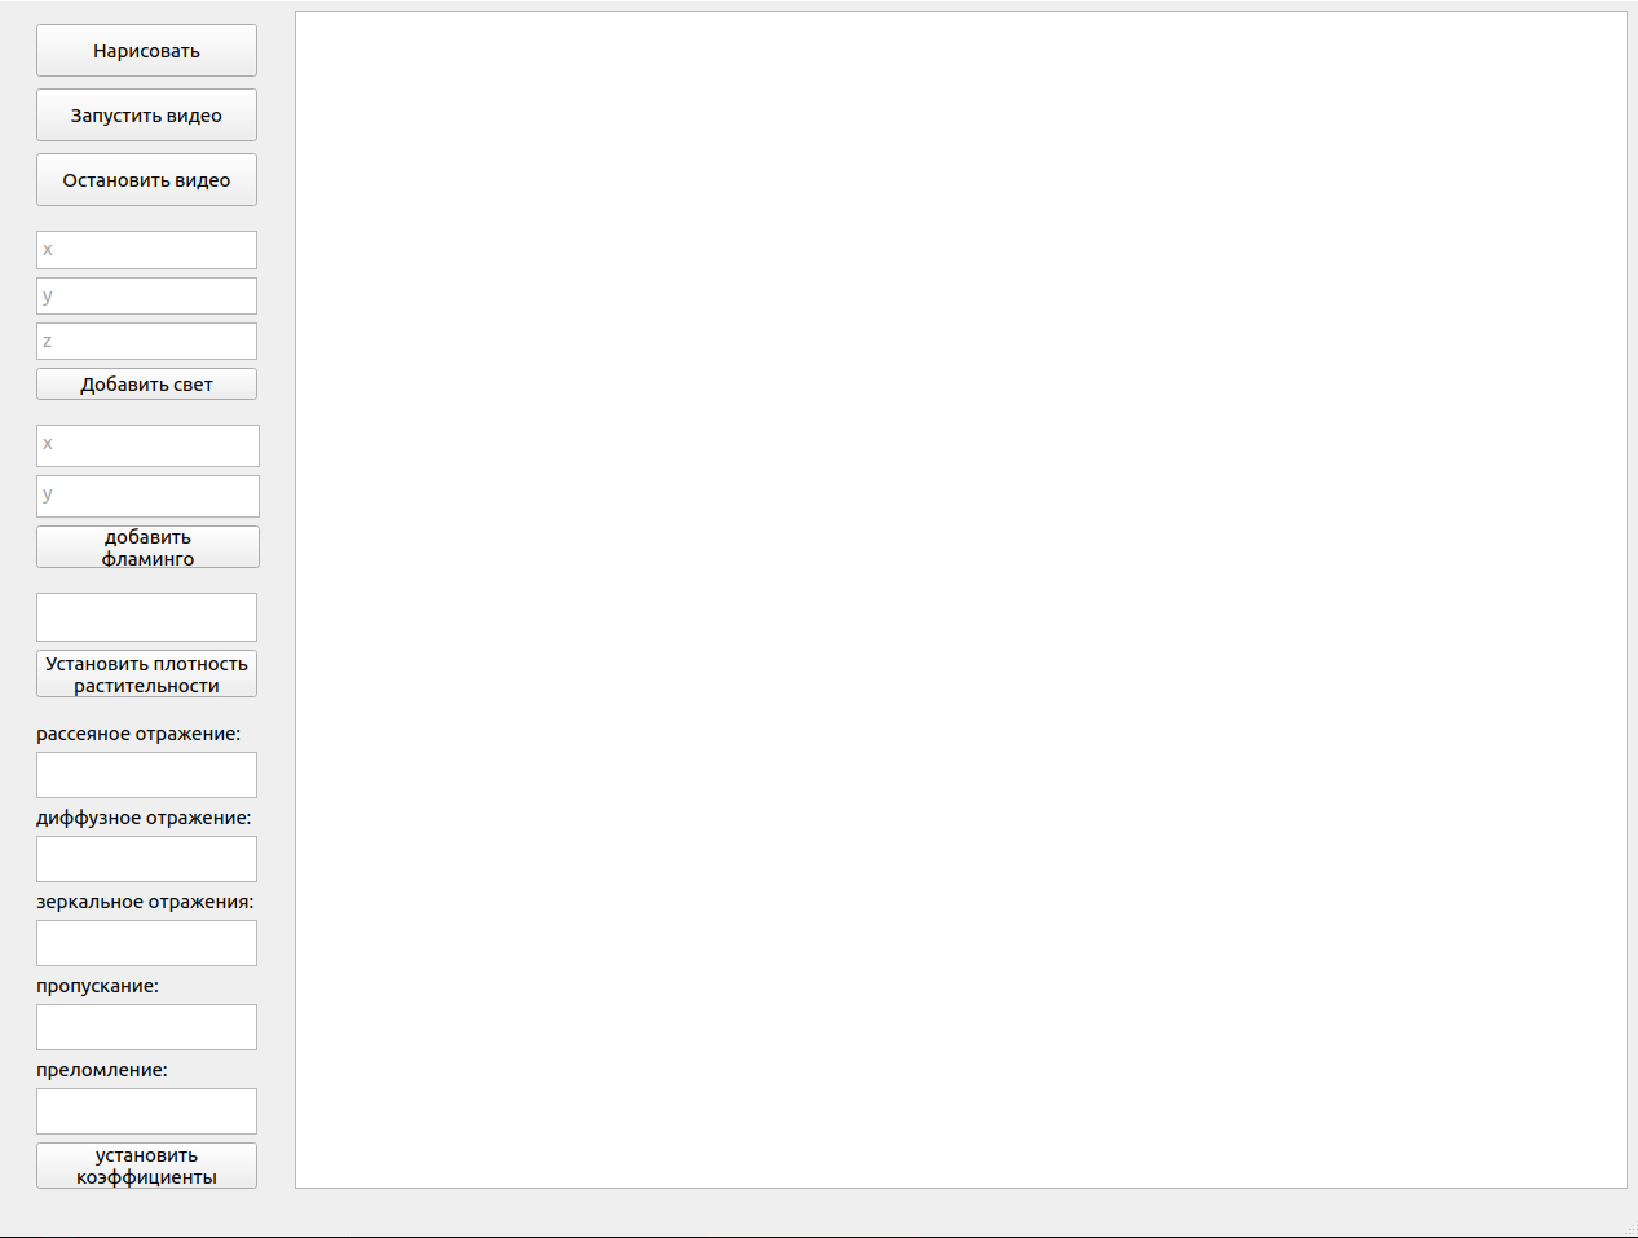
\includegraphics[width=0.96\linewidth]{img/inter}
	\caption{Пример интерфейса разработанной программы}
	\label{fig:inter}
\end{figure}

\section{Модульное тестирование}

\section{Примеры работы программы}

Примеры работы программы представлены на рисунках (\ref{fig:ex1}) и (\ref{fig:ex2}).
	
\begin{figure}[h!]
	\centering
	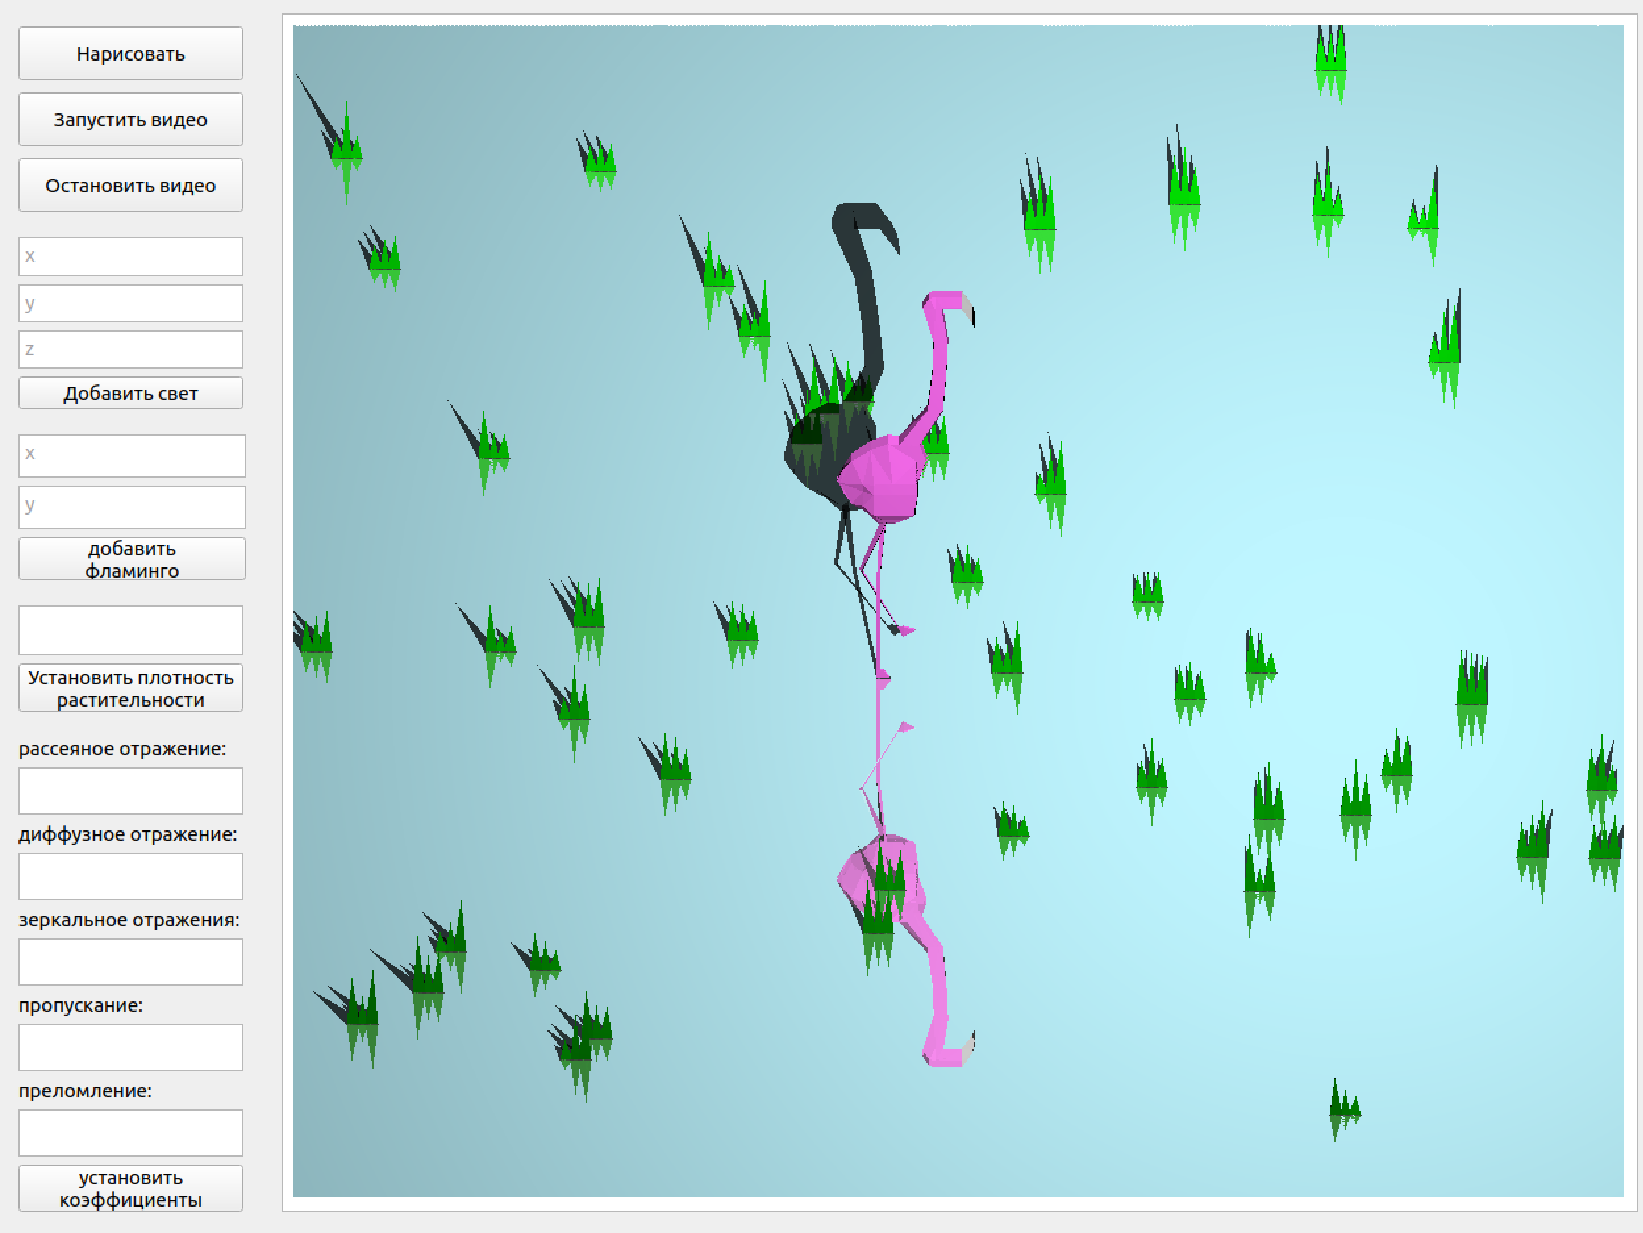
\includegraphics[width=0.9\linewidth]{img/ex1}
	\caption{Пример работы программы 1}
	\label{fig:ex1}
\end{figure}
	
\begin{figure}[h!]
	\centering
	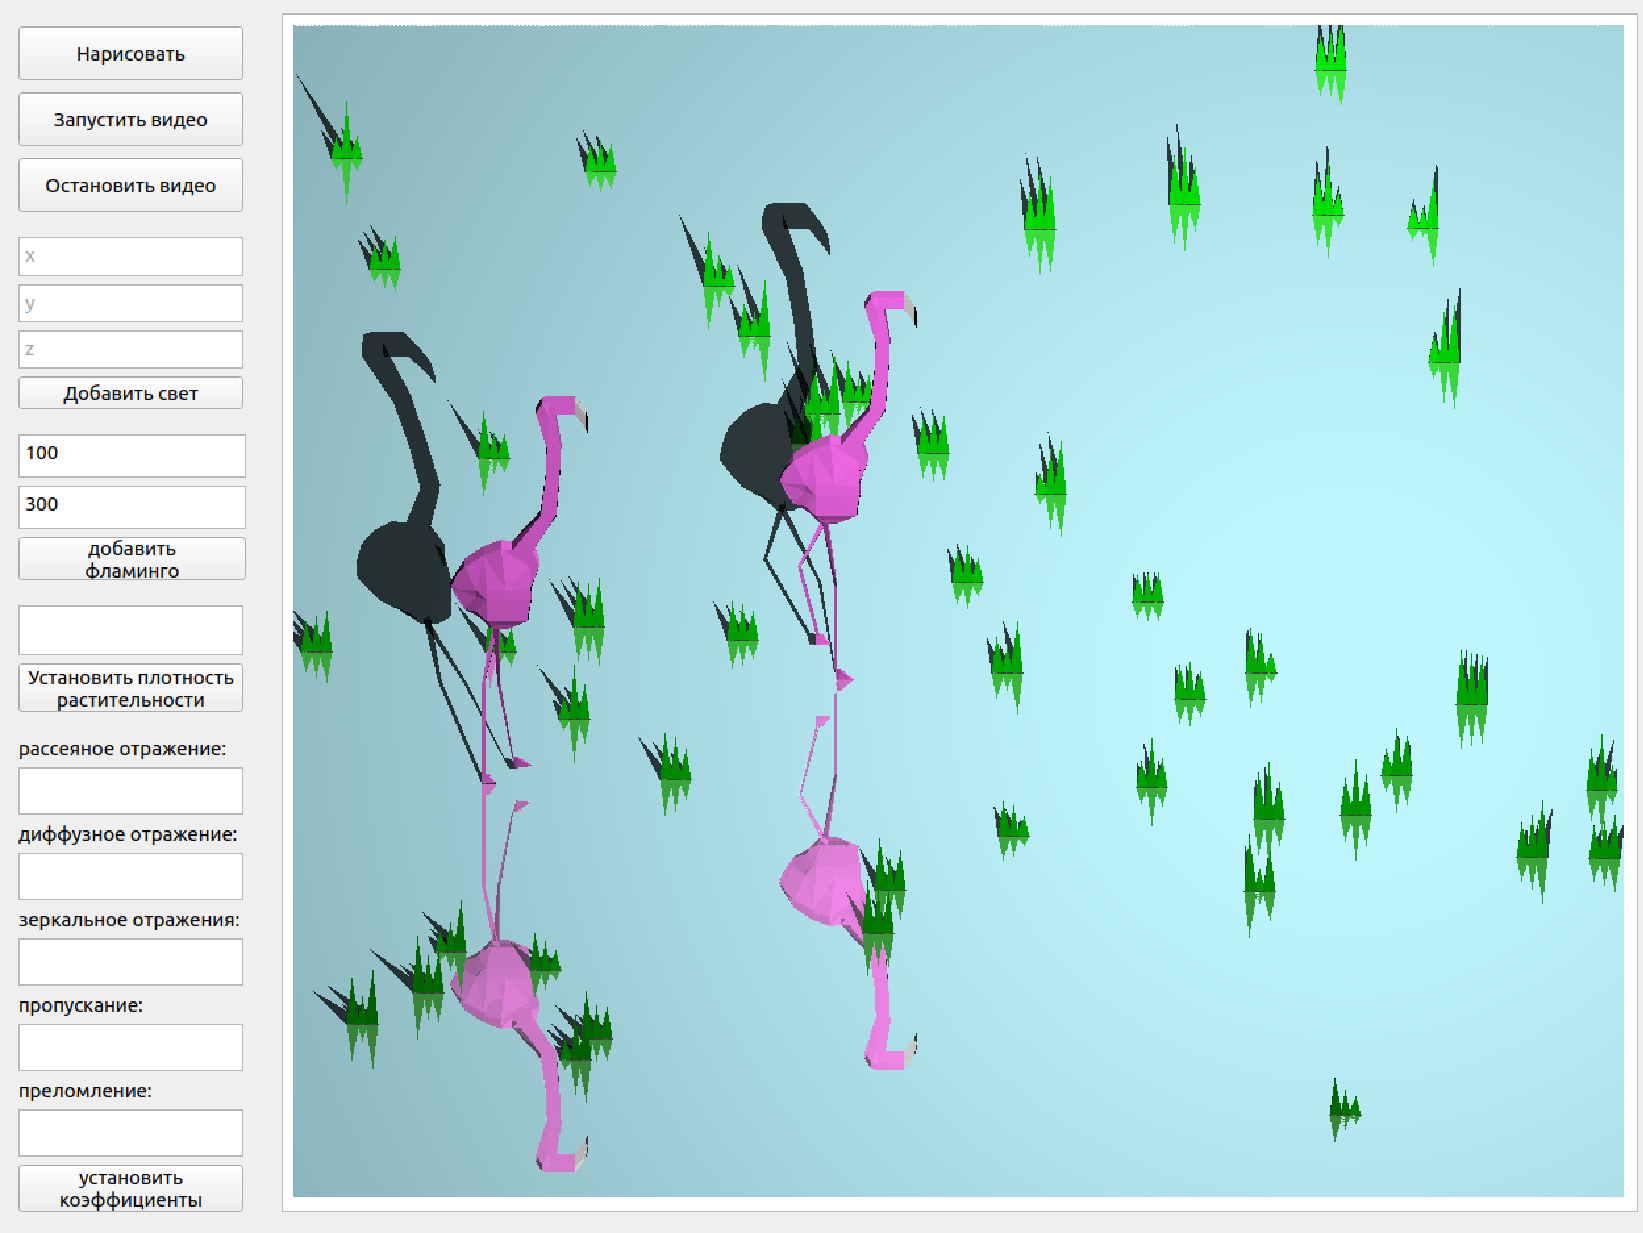
\includegraphics[width=0.9\linewidth]{img/ex2}
	\caption{Пример работы программы 2}
	\label{fig:ex2}
\end{figure}
\clearpage

\section{Функциональное тестирование}

\section{Вывод}

В данном разделе были рассмотрены средства реализации, разработано программное обеспечение, представлены листинги с реализациями основных алгоритмов программы, а также рассмотрен интерфейс и сценарии тестирования.